\chapter{Amélioration du diagnostic image}
\label{chap:chapter_5}
\chapterintro
Précédemment, nous avons tenté d'apporter une première réponse à la classification des images \gls{rcm} contenant des tissus sains, bénins ou encore malins. Nous nous sommes intéressé aux méthodes permettant de caractériser au mieux les aspects de texture de ces images par l'extraction de caractéristiques pertinentes, et nous avons employé des mécanismes permettant d'exploiter au mieux ces caractéristiques.\par

Dans ce chapitre, nous nous emploierons à améliorer la qualité du diagnostic sur les images en explorant de nouveaux schémas d'extraction de caractéristiques. Ainsi, nous pencherons sur des pistes utilisant dans un premier temps la multi-résolution et le principe de fenêtre glissante, puis dans un second temps nous envisagerons des solution de type \gls{cnn} de bout en bout et procéderons à du réglages fin de ceux-ci.\par

\newpage

\section{Méthodologie}
Lors du précédent chapitre, nous avons proposé diverses approches dans une philosophie de classification de l'image dans son intégralité pour permettre la séparation des éléments sain, bénin et malin. Cette approche suppose que l'information extraite par ces méthodes est suffisante pour permettre un diagnostic selon ces trois catégories de tissus. Cette hypothèse est partiellement juste puisqu'une même image \gls{rcm} peux comporter divers types de tissus, des trois classes précédemment évoquées, comme visible sur la \Cref{fig:scheme_annotations_hierarchy}.\par

\begin{figure}[H]
    \centering
    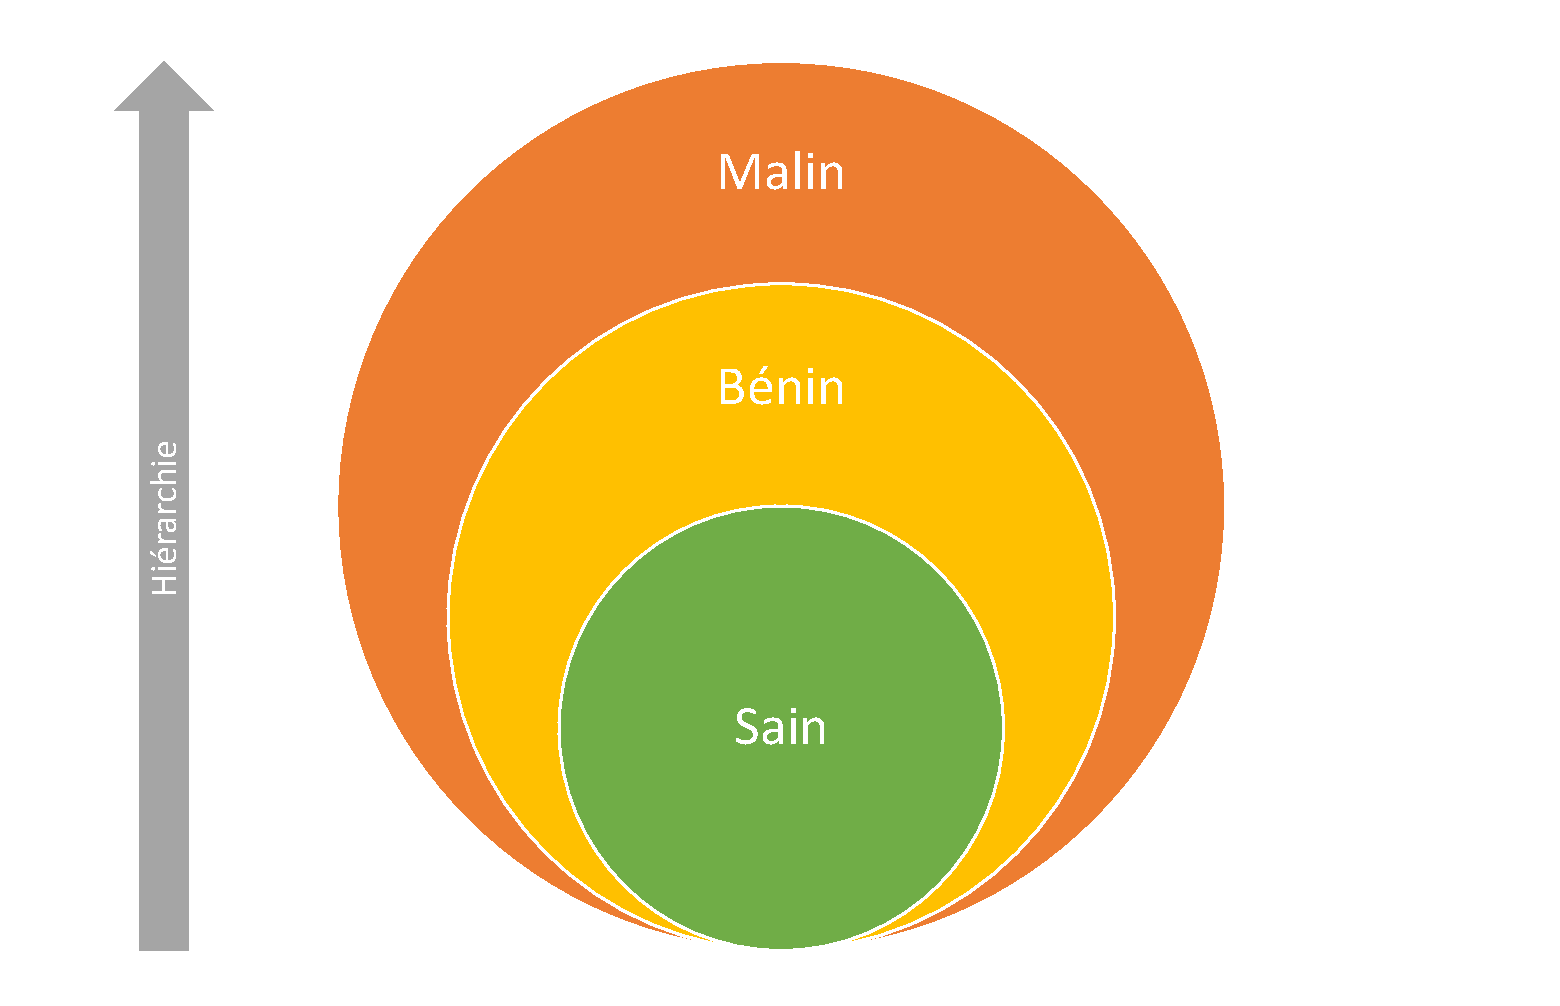
\includegraphics[width=0.7\textwidth]{contents/chapter_5/resources/scheme_annotations_hierarchy.pdf}
    \caption{Relation hiérarchiques entre les annotations. Les images malignes peuvent ainsi contenir des tissus bénin et sain ; Les images bénignes peuvent contenir des tissus sains ; Les images saines ne contiennent que des tissus sains.}
    \label{fig:scheme_annotations_hierarchy}
\end{figure}\par

Dans ce nouveau chapitre dédié à l'amélioration du diagnostic de l'image, nous exploiterons d'une part les conclusions du précèdent chapitre quant aux procédés de classification en privilégiant l'utilisation de \gls{svm} à noyau linéaire et d'autre part aux méthodes permettant l'extraction de l'information de texture. Ainsi, nous nous référerons aux méthodes suivantes :
\begin{itemize}
    \item pour la \textbf{catégorie de méthodes spatiales}, les caractéristiques définies par Haralick et al.,
    \item pour la \textbf{catégorie de méthodes spatiales}, les caractéristiques sur base d'extraction en ondelettes,
    \item pour la \textbf{catégorie de méthodes de transfert de connaissances}, nous utiliserons l'architecture ResNet.
\end{itemize}\par

Nous envisagerons de manière complémentaire des schémas alternatifs afin d'extraire une information suffisante à la séparation de nos données. Nous débuterons par la présentation de méthodes par multiples échelles, en supposant que l'information comporte plusieurs niveaux d'interprétations pouvant être capté par une méthode de classification. Dans un second temps, nous tenterons de capter l'information localement en employant un principe de fenêtres glissantes et de prédiction associées. Enfin, nous étendrons ces approches locales par l'utilisation de réseaux de \gls{cnn}, ajusté de bout en bout sur notre problème de classification à trois classes.\par
\clearpage

\section{Approche par échelles multiples}
Comme évoqué précédemment, les traitements réalisés jusqu'à lors ne permettent qu'une compréhension globale de l'image. Cette vision peux être erronée si nous supposons une compréhension à diverses échelles. Cette perspective à multiples échelles à été employée à différentes fins dans la littérature, de tâche de segmentations par exemple~\cite{Santos2012}, à des tâches de classification~\cite{Alsaih2016} ou encore de détection d'objets et d'actions~\cite{Pedersoli2011}. Nous scinderons cette section en deux parties respectives, avec d'une part l'application de ce principe à la décomposition en ondelettes et d'autres part l'application de ce principe à des techniques d'extraction spatiales.\par 

\subsection{Décomposition en ondelettes à multiples échelles}
Notre première approche par multiples échelle se portera sur la décomposition en ondelettes. En effet, ce principe a été démontré comme judicieux dans de nombreux domaines impliquant l'analyse d'images~\cite{Carvalho2004}. La décomposition peut ainsi être réalisé sous la forme d'un schéma dit diadique ou bien pyramidal. Ces deux mode sont schématisés sur la \Cref{fig:scheme_dwt_decomposition}. L'un de nos articles de référence préconise l'utilisation d'une telle méthode pour l'extraction de caractéristiques de texture sur images \gls{rcm}~\cite{Wiltgen2008}. Pour cela, cet article se focalise sur l'utilisation d'une ondelette mère de Daubechies et emploie la transformée en ondelette à cinq niveaux successifs sous forme d'arbre diadique. Les mesures associées à chaque bande de fréquences de la transformée sont les même que dans les précédent chapitre (\Cref{chap:chapter_4}) et se base sur l'extraction de la déviation standard, l'énergie et l'entropie pour un total de \textbf{39 descripteurs}. Suite aux résultats obtenus lors de précédent chapitre, nous évaluerons ce procédé par l'utilisation de l'ondelette mère de Haar et Daubechies.\par

\begin{figure}[H]
    \centering
    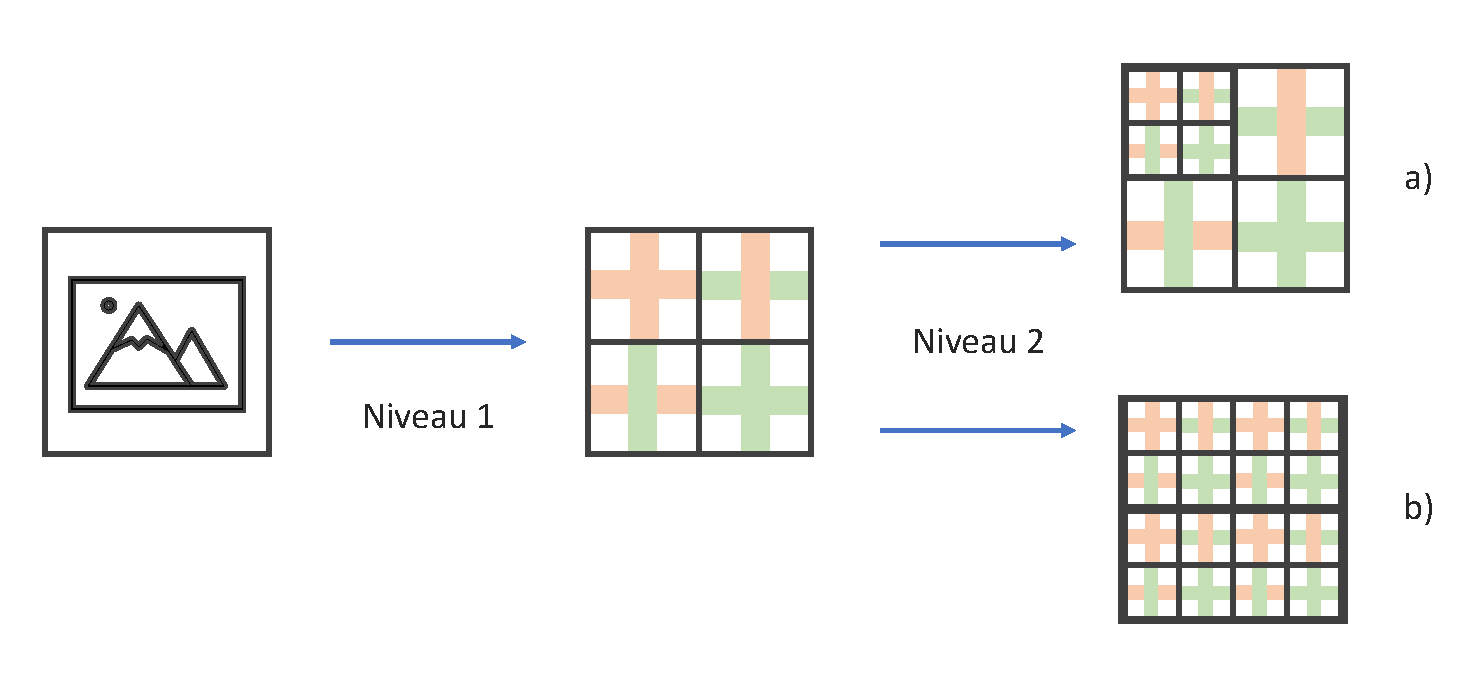
\includegraphics[width=\textwidth]{contents/chapter_5/resources/scheme_dwt_decomposition.pdf}
    \caption{Schématisation deux principaux types de décomposition successives par ondelettes. En a), schéma de décomposition multi-échelle en ondelettes dit \textbf{diadique} ; En b), schéma de décomposition multi-échelle en ondelettes dit \textbf{pyramidal}.}
    \label{fig:scheme_dwt_decomposition}
\end{figure}\par

Le second travail sur base de décomposition en ondelettes sur lequel nous nous appuyons est une extension de la transformée en ondelettes du précédent travail~\cite{Halimi2017a}. Cette transformée est réalisée de manière diadique à quatre niveaux différents de décomposition. L'auteur y propose une extraction statistique différente des précédents travaux, reposant sur une approximation à chaque niveau de décomposition par une loi normale généralisée centrée dont la densité de probabilité $f$ est décrite par l'\Cref{eq:ggd}. Les auteurs de l'étude ne retiennent comme caractéristiques que les paramètres d'échelle $\alpha$ et de forme $\beta$.\par

\begin{equation}
    f(x)= \frac{\beta}{2\alpha\Gamma(1/\beta)} e^{-\left(|\frac{x}{\alpha}|\right)^\beta}
    \label{eq:ggd}
\end{equation}

Ainsi, nos expérimentations basées sur la décomposition en ondelettes multi-échelle sont recensées sur la \Cref{tab:wavelet_multiscale_nb_features} ainsi que leurs nombres de caractéristiques associées.\par

\begin{table}[h]
    \centering
    \begin{tabular}{ll}
        \toprule
        \textbf{Méthode}                                    & \textbf{Nombre de caractéristiques}   \\ \hline
        Ondelettes - Haar                                   & 39 (13$\times$3)   \\ \hline
        Ondelettes - Daubechies / Wiltgen~\cite{Wiltgen2008}& 39 (13$\times$3)   \\ \hline
        Halimi~\cite{Halimi2017a}                           & 24 (12$\times$2)   \\
        \bottomrule
    \end{tabular}
    \caption{Listes des méthodes sur base de décomposition multi-échelle en ondelettes et nombre de caractéristiques extraites.}
    \label{tab:wavelet_multiscale_nb_features}
\end{table}\par

\subsection{Approche par échelles multiples}
Toujours dans cette optique d'approche multi-échelle, divers travaux se sont orientées afin de permettre une classification d'images médicale sur base d'extraction de caractéristiques spatiale multi-échelle~\cite{Alsaih2016,Tzalavra2016}. 
Nous intéresserons essentiellement à ceux-ci dans cette partie. Nous avions lors du précédent chapitre, cité le travail de Wiltgen, qui semble le travail le plus proche en terme de multi échelle appliqué à des images ~\gls{rcm} de dermatologie~\cite{Wiltgen2008}.\par

\begin{figure}[H]
    \centering
    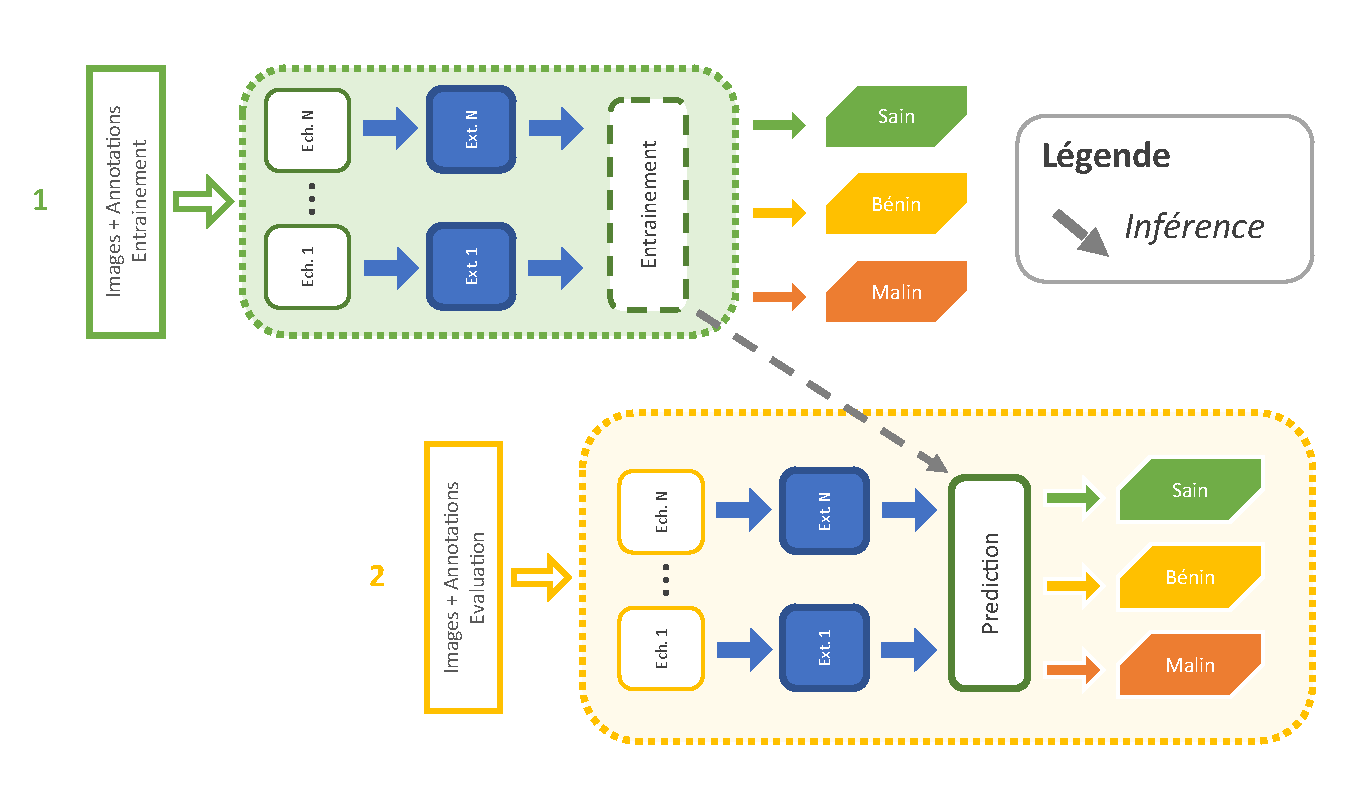
\includegraphics[width=\linewidth]{contents/chapter_5/resources/scheme_multiscale_features.pdf}
    \caption{Schéma de représentation du système multi-échelles sur base d'extraction puis de agrégation des caractéristiques avant classification.}
    \label{fig:scheme_multiscale_features}
\end{figure}\par

Ainsi, nous mettrons en oeuvre deux processus multi échelle dans ce chapitre. Le premier d'entre eux, de basera sur une approche de type fusion de caractéristiques avant l'étape de classification, tel qu'utilisé dans des travaux à but similaire~\cite{Pedersoli2011,Alsaih2016}. Ce principe est schématisé au travers de la \Cref{fig:scheme_multiscale_features}. Notre seconde proposition correspondra à une classification en deux temps. En effet, nous considérerons la spécialisation de classifieur à une échelle précise, et tenterons d'amener à une fusion de la décision tel que présenté sur la \Cref{fig:scheme_multiscale_decision}.\par

\begin{figure}[H]
    \centering
    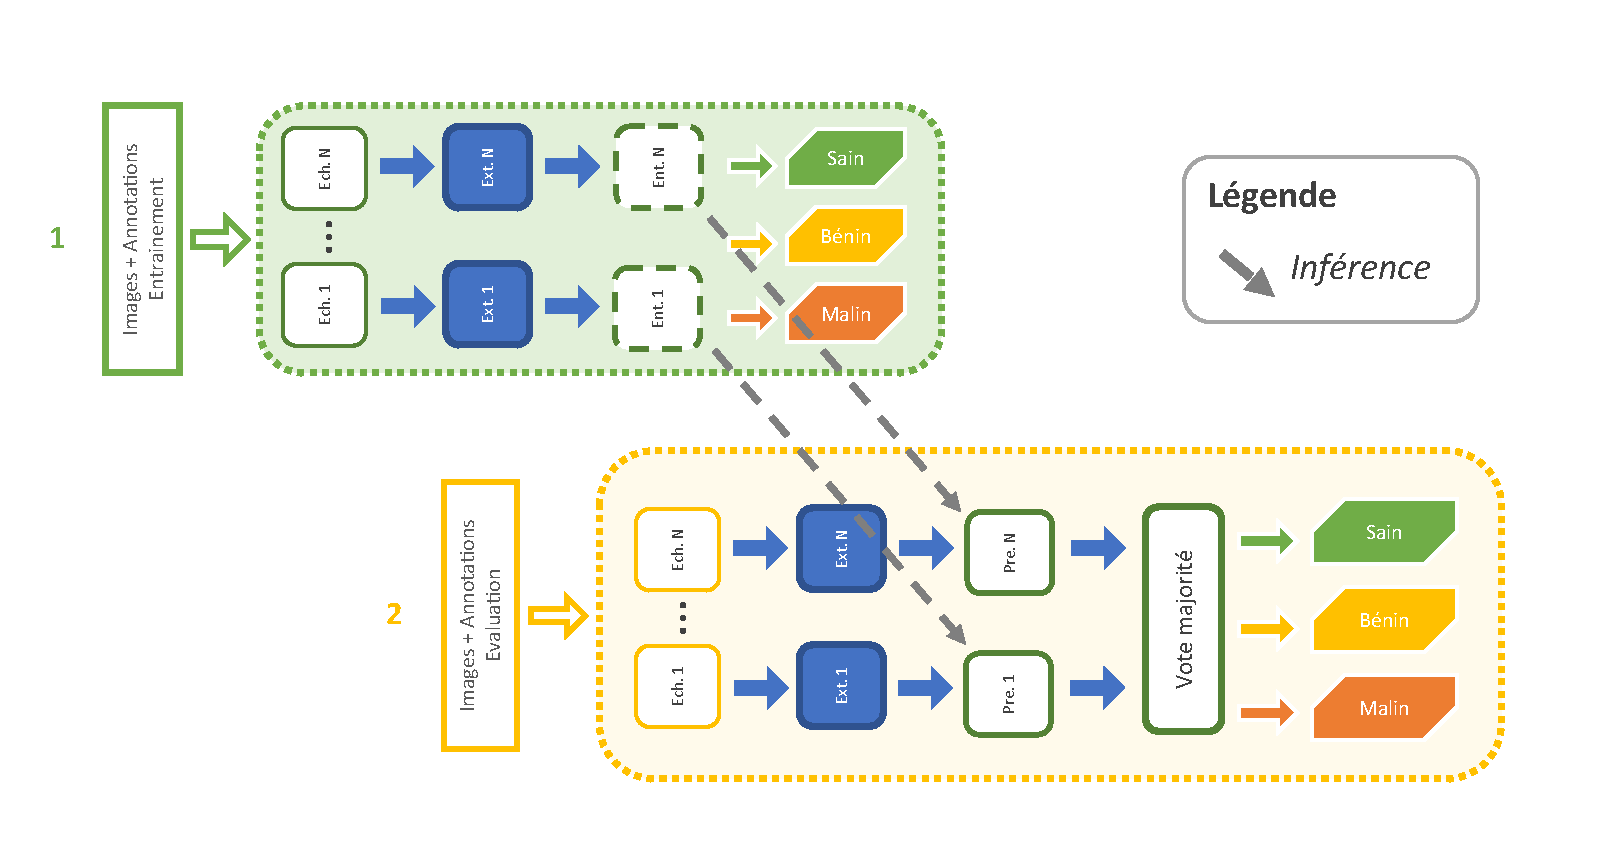
\includegraphics[width=\linewidth]{contents/chapter_5/resources/scheme_multiscale_decision.pdf}
    \caption{Schéma de représentation du système multi-échelles, sur base d'extractions et de classification à chaque échelle respective et par agrégation des décisions.}
    \label{fig:scheme_multiscale_decision}
\end{figure}\par

\section{Approche par fenêtre glissante}
Ces types d'approches ont été récemment utilisées à but de détection spatiale d'objet par l'utilisation de méthode d'apprentissage profond. A des fins médicales, ces approches ont permis la détection sur des images \gls{mri} du ventricule gauche~\cite{Helwan2017}.\par

Ces approches peuvent être également utilisées dans un contexte de classification lorsque la donnée comporte de l'information non directement liée aux annotations finales comme pour de la détection de cancer sur images histologiques par exemple~\cite{Hou2016,Alqudah2019}.\par

Les données images en notre possession corroborent avec ce type de schéma, puisque celle-ci sont soumise à un label global pour lesquels une hiérarchie à été mise en place. Pour rappel, un label malin qualifiera une donnée comportant au minimum des tissus typique d'une pathologie maligne mais pourra également comporter des tissus bénin et sain, et une annotation bénigne ne comportera que des tissus bénin ou sain.\par

Nous opterons pour un schéma de type supervisé de type approche de détection à faible échelle suivi d'une agrégation des décisions tel qu'employé dans certains travaux~\cite{Alqudah2019}. En effet, les données en notre possession nous permettent l'accès à des annotations de tissus de plus bas niveau réalisées par un spécialiste selon les même trois critères d'annotation.\par

Afin de mettre en oeuvre le schéma de détection à basse échelle, nous appliquerons les techniques jugées les plus pertinentes du chapitre précédent. Nous emploierons pour cela un schéma de classification comme sur la \Cref{fig:scheme_multiscale_decision}. De plus, n'ayant pas de critères de tailles optimum, nous feront varier ces paramètres afin d'étudier leur impact sur la classification. ces paramètres sont visible sur la \Cref{tab:sliding_window_parameters}.\par

\begin{figure}[H]
    \centering
    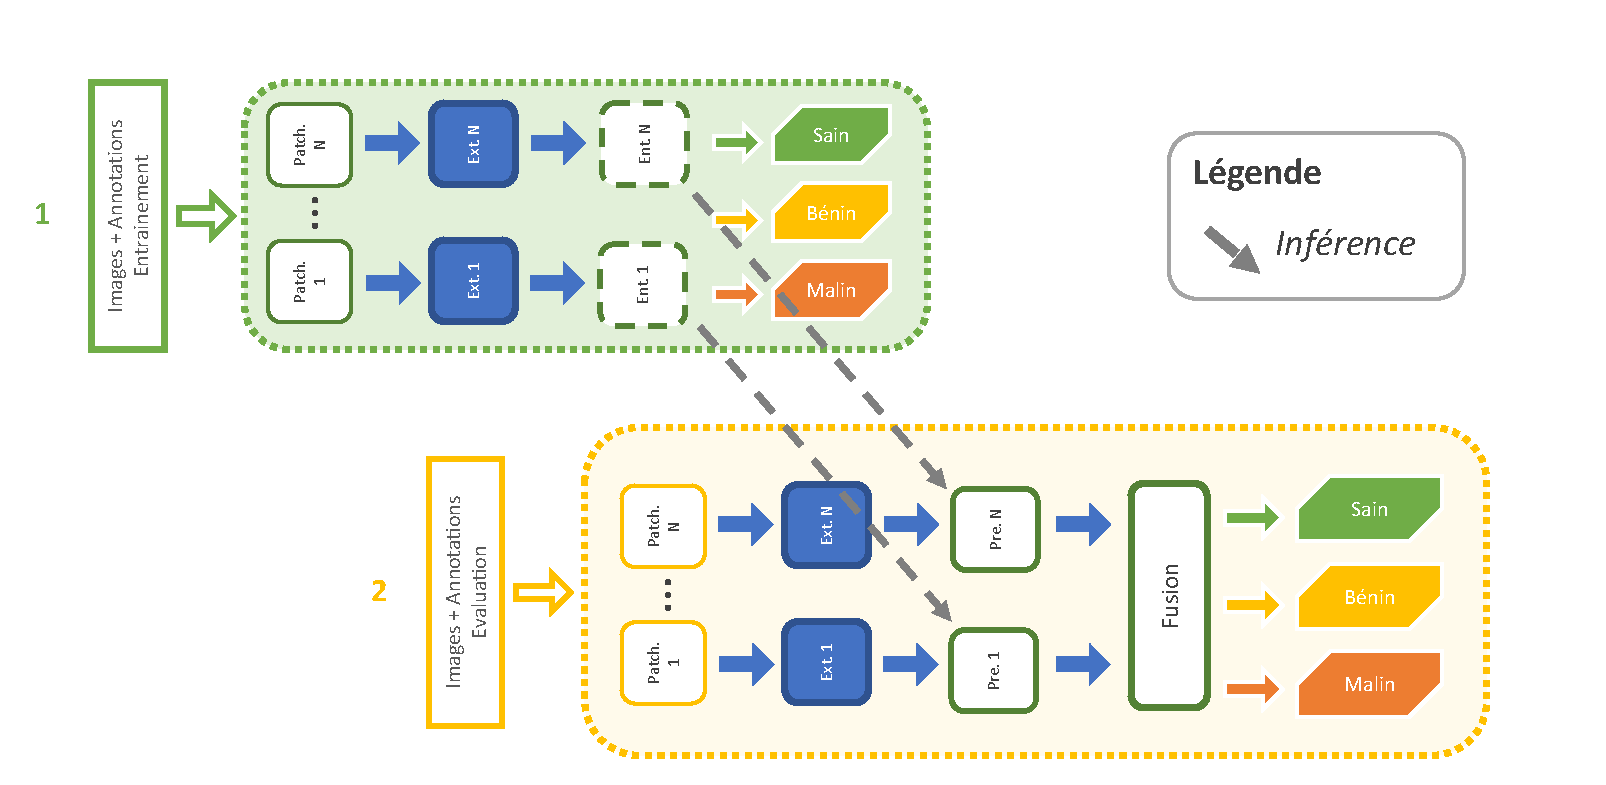
\includegraphics[width=\linewidth]{contents/chapter_5/resources/scheme_sliding_features.pdf}
    \caption{Schéma de représentation du système multi-échelles, sur base d'extractions et de classification à chaque échelle respective et par agrégation des décisions.}
    \label{fig:scheme_sliding_features}
\end{figure}\par

\begin{table}[H]
    \centering
    \begin{tabular*}{0.6\linewidth}{l@{\extracolsep{\fill}}l}
    \toprule
    \textbf{Résolution spatiale}& \textbf{Chevauchement}   \\ \hline
    250*250                     & 0\%                      \\ \hline
    250*250                     & 25\%                     \\ \hline
    250*250                     & 50\%                     \\ \hline 
    500*500                     & 0\%                      \\ \hline
    500*500                     & 25\%                     \\ \hline
    500*500                     & 50\%                     \\
    \bottomrule
    \end{tabular*}
    \caption{Paramètres appliqués à l'approche par fenêtre glissante.}
    \label{tab:sliding_window_parameters}
\end{table}\par

\section{Réglage fin de réseaux de convolution}
Dans cette partie, nous considérerons l'utilisation du réglage fin des \gls{cnn} adapté à notre problématique de classification d'images \gls{rcm}. Pour cela, nous nous consacrerons à ses divers aspects à l'aide de sous parties respectives propre à chaque concept. Nous débuterons par une présentation du réglage fin et des architectures que nous considérerons. Puis nous aborderons diverses techniques que nous mettrons en oeuvre, dont :
\begin{inlinerate}
    \item l'augmentation de données,
    \item le programme d'apprentissage,
    \item et la fonction de coût.
\end{inlinerate}\par

\subsection{Présentation générale}
Le réglage fin est une extension de l'apprentissage par transfert dans lequel est ajouté une ou des couches de classification adaptées au problème traité, et dans lequel tout ou partie du réseau est ré-entraîné à partir des poids existants. Ce mode d'apprentissage est utilisé lorsque les données propre au nouveau problème sont suffisantes, et permet d'obtenir un réseau plus adapté au nouveau problème.\par

Concernant les architectures que nous évaluerons dans ce chapitre, le travail mené par Park~\cite{Park2019} privélgie l'utilisation d'une architecture ResNet 50~\cite{He2016}. Néanmoins, lors du \Cref{chap:chapter_4} nous avons pu déterminer que l'architecture Inception-ResNet~\cite{Szegedy2017} utilisant un couche de Global Average Pooling et pré-entraîné sur la base ImageNet, semblait la plus judicieuse pour la classification de nos données.\par

A ce propos, aucune information n'est stipulée sur le type de Pooling employé par ce travail~\cite{Park2019}. Nous pouvons supposer l'utilisation d'une couche de Global Pooling basé sur la moyenne, couramment utilisée notamment pour de la visualisation de \gls{cnn} comme le propose ce travail.\par

\subsection{Augmentation de données}
Nous parlerons dans cette partie d'augmentation de données au sens de traitements appliqués au données d'entrées et non de création d'échantillons virtuels à partir de l'espace des caractéristiques pour corriger les problèmes de balancements~\cite{Wong2016}. Ainsi, nous considérerons l'augmentation de données comme une technique permettant de contrer le sur-apprentissage dans ce travail.\par


Ainsi, cette transformation est appliquée aux données d'entraînement afin d'apporter des variations.\par

~\cite{taylor2018}
\subsection{Programme d'apprentissage}
Le programme d'apprentissage ou \textit{Curriculum Learning} est une démarche visant par analogie à l'humain, à entraîner tout \gls{cnn} en proposant diverses tâches intermédiaires avec une difficulté croissante, afin d'accomplir avec une plus grande efficacité une tâche plus complexe. La raison technique recherché par cette méthode, est de proposer un espace de recherche plus simples des afin de trouver un meilleur minimum local comme l'ont suggéré ses premiers auteurs~\cite{Bengio2009}.\par

De récents travaux sur des images médicales, issue de rayons X (images en niveau de gris) ont permis par cette approche d'augmenter les performance de détection de \gls{cnn} sur des cancer du sein~\cite{Lotter2017} ou encore des cancers et autres pathologies pulmonaires~\cite{Park2019}. Le principe suivi par ces deux travaux, est de procéder à l'extraction de sous images de taille restreinte autour des dites lésions avérées, mais gardant la même propriété d'échelle. En effet, la gestion d'une même donnée à échelles multiples sur \gls{cnn} est un problème largement traité de la littérature non aisé~\cite{Noord2017}.\par

Ainsi nous emploierons à cet effet notre base d'images originale couplé aux sous images associées pour gérer cette tâche.\par

\subsection{Fonction de coût}
La fonction de coût est autre aspect que nous avons tenté de mener à bien dans ce travail.
~\cite{Park2019}
~\cite{Barbu2018}

\subsection{Carte d'activation de classe}
~\cite{jia2017}
\section{Analyse des résultats}

\begin{table}[H]
    \centering
    \begin{tabular}{llll}
        \toprule
        Catégories                  & Méthodes                  & 3 Classes         & Malin             \\ \midrule
        \multirow{3}{*}{Ondelettes} & Haar                      & 0.65±0.08         & 0.70±0.06         \\
                                    & Wiltgen~\cite{Wiltgen2008}& \textbf{0.66±0.06}& \textbf{0.71±0.06}\\
                                    & Halimi~\cite{Halimi2017a} & 0.38±0.02         & 0.41±0.04         \\ \midrule
        \multirow{5}{*}{Spatial}    & Fusion de caractéristiques& \textbf{0.63±0.06}& 0.66±0.07         \\
                                    & Décisions - Maximum       & 0.60±0.10         & 0.64±0.08         \\
                                    & Scores - Moyenne + Maximum& 0.60±0.10         & \textbf{0.67±0.07}\\
                                    & Scores - Maximum + Maximum& 0.59±0.10         & 0.65±0.08         \\
                                    & Scores - \gls{svm} Linéaire& 0.57±0.10        & 0.65±0.04         \\ \midrule
        \multirow{5}{*}{Transfert}  & Fusion de caractéristiques& \textbf{0.76±0.06}& \textbf{0.83±0.02}\\
                                    & Décisions - Maximum       & 0.69±0.10         & 0.78±0.05         \\
                                    & Scores - Moyenne + Maximum& 0.69±0.11         & 0.79±0.06         \\
                                    & Scores - Maximum + Maximum& 0.69±0.11         & 0.79±0.06         \\
                                    & Scores - \gls{svm} Linéaire& 0.72±0.04        & 0.79±0.03         \\
        \bottomrule
    \end{tabular}
    \label{tab:image_improvement_multiresolution}
    \caption{Résultats issus du processus de classification basé sur la classification multi-échelles.}
\end{table}


\begin{landscape}

\begin{table}[H]
    \centering
    \begin{tabular}{cclllllll}
		\toprule
		\multirow{2}{*}{Taille}     & \multirow{2}{*}{Superposition}    & \multirow{2}{*}{Mode}     & \multicolumn{2}{c}{Spatial}       & \multicolumn{2}{c}{Fréquence}     & \multicolumn{2}{c}{Transfert}         \\
		                            &                                   &                           & 3 Classes         & Malin         & 3 Classes         & Malin         & 3 Classes         & Malin             \\ \midrule
		250                         & Aucun                             & Patch                     & 0.67±0.10         & 0.41±0.13     & 0.72±0.07         & 0.44±0.10     & \textbf{0.91±0.02}& \textbf{0.82±0.03}\\ \midrule
		\multirow{12}{*}{250}       & \multirow{4}{*}{0}                & D\_ALO                    & 0.52±0.02         & 0.67±0.04     & 0.44±0.06         & 0.65±0.05     & 0.58±0.04         & 0.71±0.05         \\ 
							        &                                   & D\_DYN                    & 0.62±0.02         & 0.68±0.05     & 0.57±0.06         & 0.67±0.04     & 0.75±0.02         & 0.80±0.03         \\
							        &                                   & S\_MAX\_DYN               & 0.54±0.02         & 0.63±0.04     & 0.50±0.08         & 0.66±0.05     & 0.70±0.03         & 0.76±0.02         \\
							        &                                   & S\_SVC                    & 0.60±0.05         & 0.66±0.04     & 0.59±0.08         & 0.65±0.07     & 0.78±0.03         & 0.81±0.03         \\ \cline{2-9}
							        & \multirow{4}{*}{25}               & D\_ALO                    & 0.49±0.10         & 0.67±0.10     & 0.41±0.10         & 0.65±0.10     & 0.53±0.05         & 0.70±0.09         \\
							        &                                   & D\_DYN                    & 0.62±0.07         & 0.68±0.11     & 0.58±0.08         & 0.66±0.09     & 0.75±0.03         & 0.80±0.04         \\
							        &                                   & S\_MAX\_DYN               & 0.52±0.03         & 0.59±0.06     & 0.49±0.08         & 0.66±0.10     & 0.72±0.04         & 0.78±0.03         \\
							        &                                   & S\_SVC                    & 0.62±0.06         & 0.71±0.06     & 0.57±0.10         & 0.66±0.08     & 0.78±0.03         & 0.81±0.03         \\ \cline{2-9}
							        & \multirow{4}{*}{50}               & D\_ALO                    & 0.46±0.11         & 0.66±0.08     & 0.39±0.12         & 0.64±0.08     & 0.49±0.10         & 0.68±0.08         \\
							        &                                   & D\_DYN                    & 0.62±0.03         & 0.68±0.07     & 0.59±0.10         & 0.67±0.08     & 0.75±0.03         & 0.80±0.03         \\
							        &                                   & S\_MAX\_DYN               & 0.52±0.06         & 0.63±0.07     & 0.49±0.10         & 0.65±0.07     & 0.72±0.03         & 0.80±0.01         \\ 
		                            &                                   & S\_SVC                    & 0.61±0.08         & 0.69±0.08     & 0.61±0.07         & 0.68±0.06     & \textbf{0.78±0.03}& \textbf{0.82±0.02}\\ \midrule
		\multirow{12}{*}{500}       & \multirow{4}{*}{0}                & D\_ALO                    & 0.58±0.08         & 0.63±0.05     & 0.23±0.11         & 0.00±0.00     & 0.74±0.05         & 0.76±0.05         \\
							        &                                   & D\_DYN                    & 0.59±0.04         & 0.63±0.05     & 0.28±0.05         & 0.63±0.05     & 0.72±0.05         & 0.76±0.05         \\
							        &                                   & S\_MAX\_DYN               & 0.50±0.05         & 0.56±0.15     & 0.53±0.08         & 0.66±0.04     & 0.70±0.03         & 0.78±0.04         \\
							        &                                   & S\_SVC                    & 0.59±0.08         & 0.67±0.07     & 0.36±0.04         & 0.55±0.17     & 0.69±0.13         & 0.74±0.08         \\ \cline{2-9}
							        & \multirow{4}{*}{25}               & D\_ALO                    & 0.55±0.08         & 0.64±0.07     & 0.23±0.11         & 0.00±0.00     & 0.77±0.05         & 0.80±0.04         \\
							        &                                   & D\_DYN                    & 0.55±0.10         & 0.63±0.05     & 0.28±0.05         & 0.63±0.05     & 0.76±0.04         & 0.80±0.04         \\
							        &                                   & S\_MAX\_DYN               & 0.53±0.03         & 0.55±0.09     & 0.54±0.07         & 0.67±0.05     & 0.73±0.03         & 0.80±0.04         \\
							        &                                   & S\_SVC                    & 0.58±0.07         & 0.67±0.06     & 0.37±0.04         & 0.55±0.18     & 0.77±0.05         & 0.81±0.04         \\ \cline{2-9}
							        & \multirow{4}{*}{50}               & D\_ALO                    & 0.57±0.08         & 0.67±0.11     & 0.23±0.07         & 0.00±0.00     & 0.77±0.03         & 0.81±0.05         \\
							        &                                   & D\_DYN                    & 0.58±0.07         & 0.67±0.11     & 0.28±0.12         & 0.63±0.12     & 0.76±0.03         & 0.80±0.05         \\
							        &                                   & S\_MAX\_DYN               & 0.52±0.05         & 0.55±0.06     & 0.55±0.07         & 0.67±0.13     & 0.73±0.04         & 0.80±0.05         \\
		                            &                                   & S\_SVC                    & 0.60±0.06         & 0.65±0.09     & 0.34±0.05         & 0.39±0.23     & \textbf{0.78±0.02}& \textbf{0.81±0.04}\\
		\bottomrule
    \end{tabular}
    \label{tab:image_improvement_sliding_window}
    \caption{Résultats issus du processus de classification basé sur les fenêtres glissantes.}
\end{table}

\end{landscape}

\begin{table}[H]
    \centering
    \begin{tabular}{llll}
        \toprule
        Catégorie                   & Pooling           & 3 Classes         & Malin             \\ \midrule
        \multirow{2}{*}{Réglage fin}& Fonction moyenne  & 0.44±0.05         & 0.69±0.06         \\
                                    & Fonction maximum  & \textbf{0.56±0.05}& \textbf{0.78±0.05}\\
        Réglage fin + Programme     & Fonction maximum  & 0.51±0.07         & 0.67±0.05         \\
        \bottomrule
    \end{tabular}
    
    \label{tab:image_improvement_fine}
    \caption{Résultats issus du processus de classification basé sur les \gls{cnn} par réglages fin et programme d'apprentissage.}
\end{table}